\chapter{Pharmacological Class}
The three drugs Chlordiazepoxide, diazepam, and lorazepam belong to a class of drugs named benzodiazepines\footnote{BZD, BZs or benzos}

\section{Chemical Structure}
Benzodiazepines consist of a benzene ring attached to diazepine ring.
The chlordiazepoxide has an (N-methylamine) substitued on position 2, an oxygen on position $4$, and a chlorine atom on postion 7 on the benzodiazepine.
Diazepam has a methyl group on position 1, an oxygen on position 2, and a chlorine on position 7.
Lorazepam has an oxygen on position 2, a hydroxyl on position 3, a chlorine on position $2'$.

Benzodiazepines are a class of psychoactive drugs. that enhance the effect of \emph{\uppercase{gaba}} at the \emph{GABA$_A$} receptor which results in sedative, hypnotic, anxiolytic, anticonvulsant, muscle relaxant properties.

Benzodiazepines are used in treating anxiety, insomnia, agitation, sezures, muscle spasms, alcohol withdrawal.\cite{}


The structures of Chlordiazepoxide \emph{Fig} \ref{fig:cldiazepoxide}, Diazepam \emph{Fig} \ref{fig:diazepam}, and Lorazepam \emph{Fig} \ref{fig:lorazepam} consist of the major structure of the benzodiazepine \emph{Fig} \ref{fig:benzo} substituted on different atoms to give the many variants. The numbering \footnote{Long story short, We start from the fused rings, at the atom adjacent to the fusion point on the bigger ring that is closest to a heteroatom, we then go around the ring and increase the number. We usually do not include the atoms that are included in the fusion as they are rarely substitued. The benzene ring takes numbering as conventional with the carbon at the attachment point takes number $1'$} is based on the \emph{IUPAC} \footnote{International Union of Pure and Applied Chemistry}.

%How to make a space between figures
	\begin{figure}
		\centering
		\begin{minipage}{.5\textwidth}
			\centering
			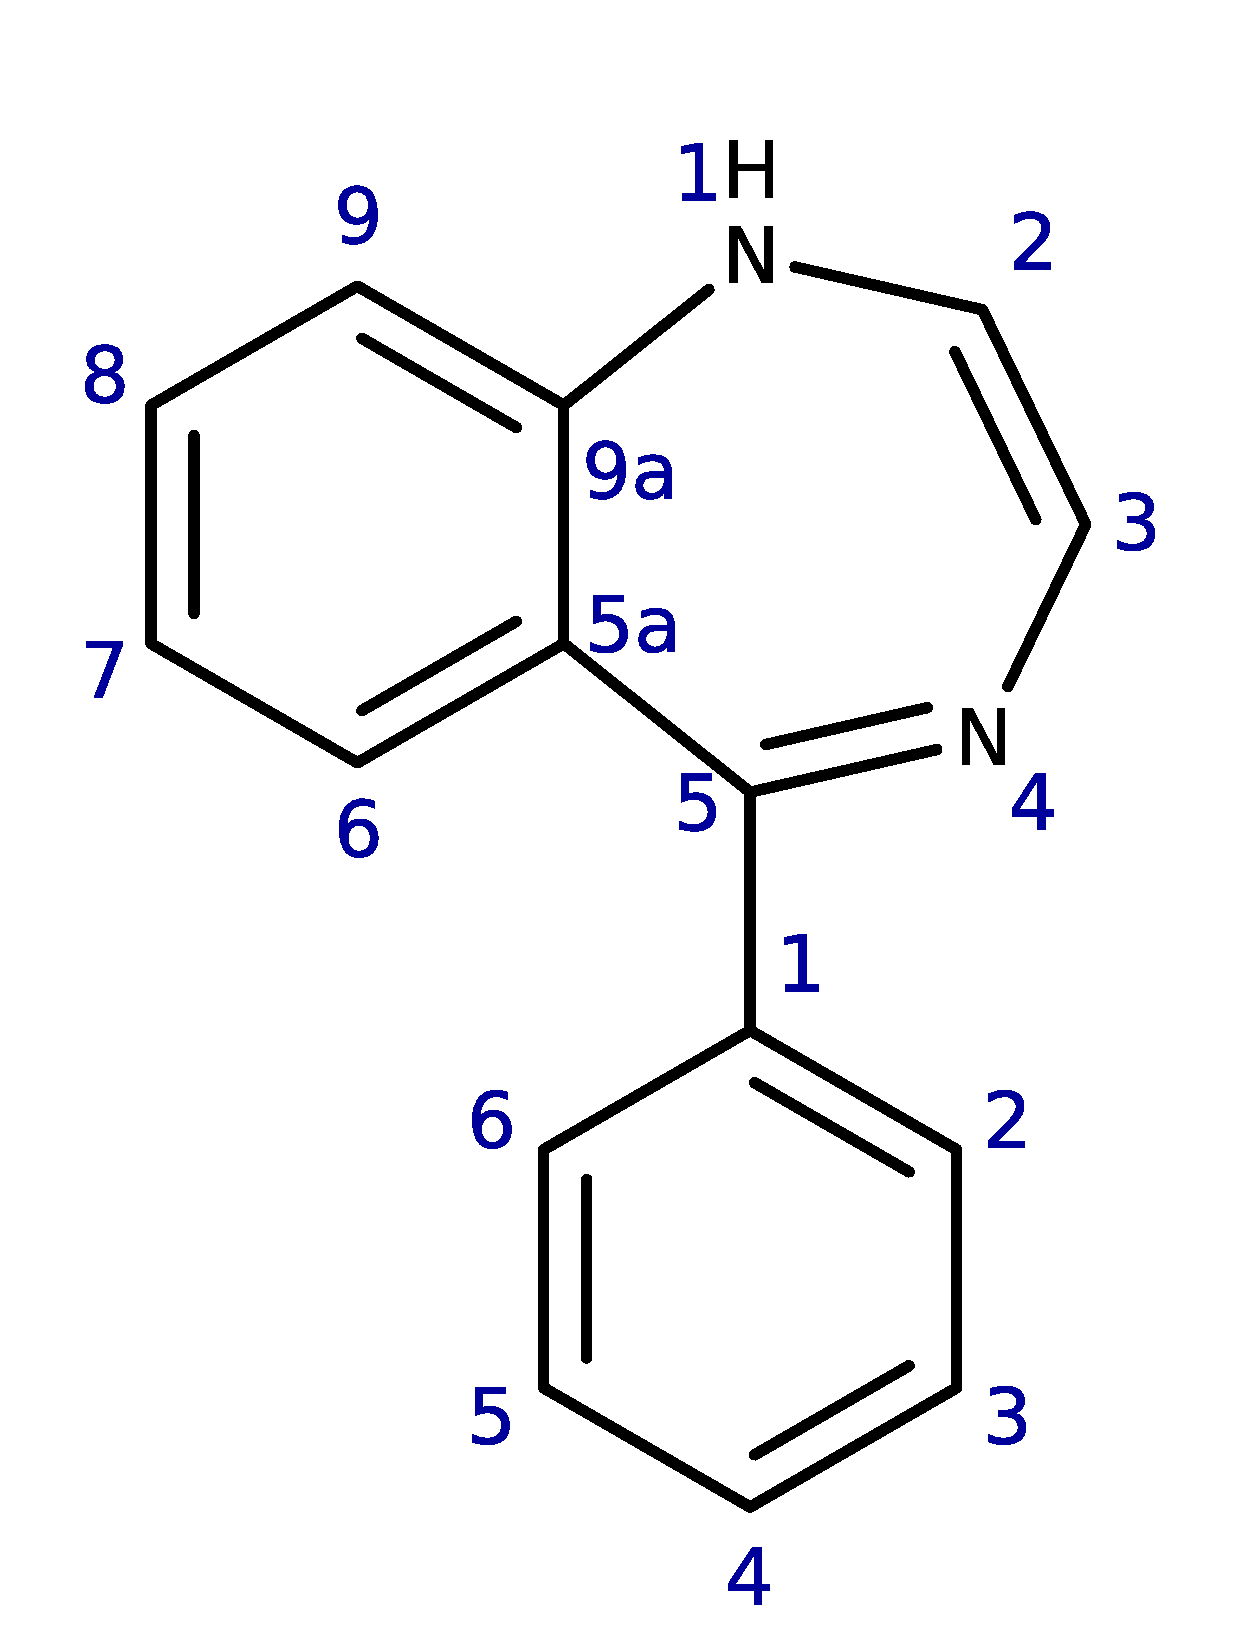
\includegraphics[width=\linewidth]{benzo.pdf}
			\captionof{figure}{Typical Structure of the Benzodiazepines}
			\label{fig:benzo}
		\end{minipage}%
		\begin{minipage}{.5\textwidth}
			\centering
			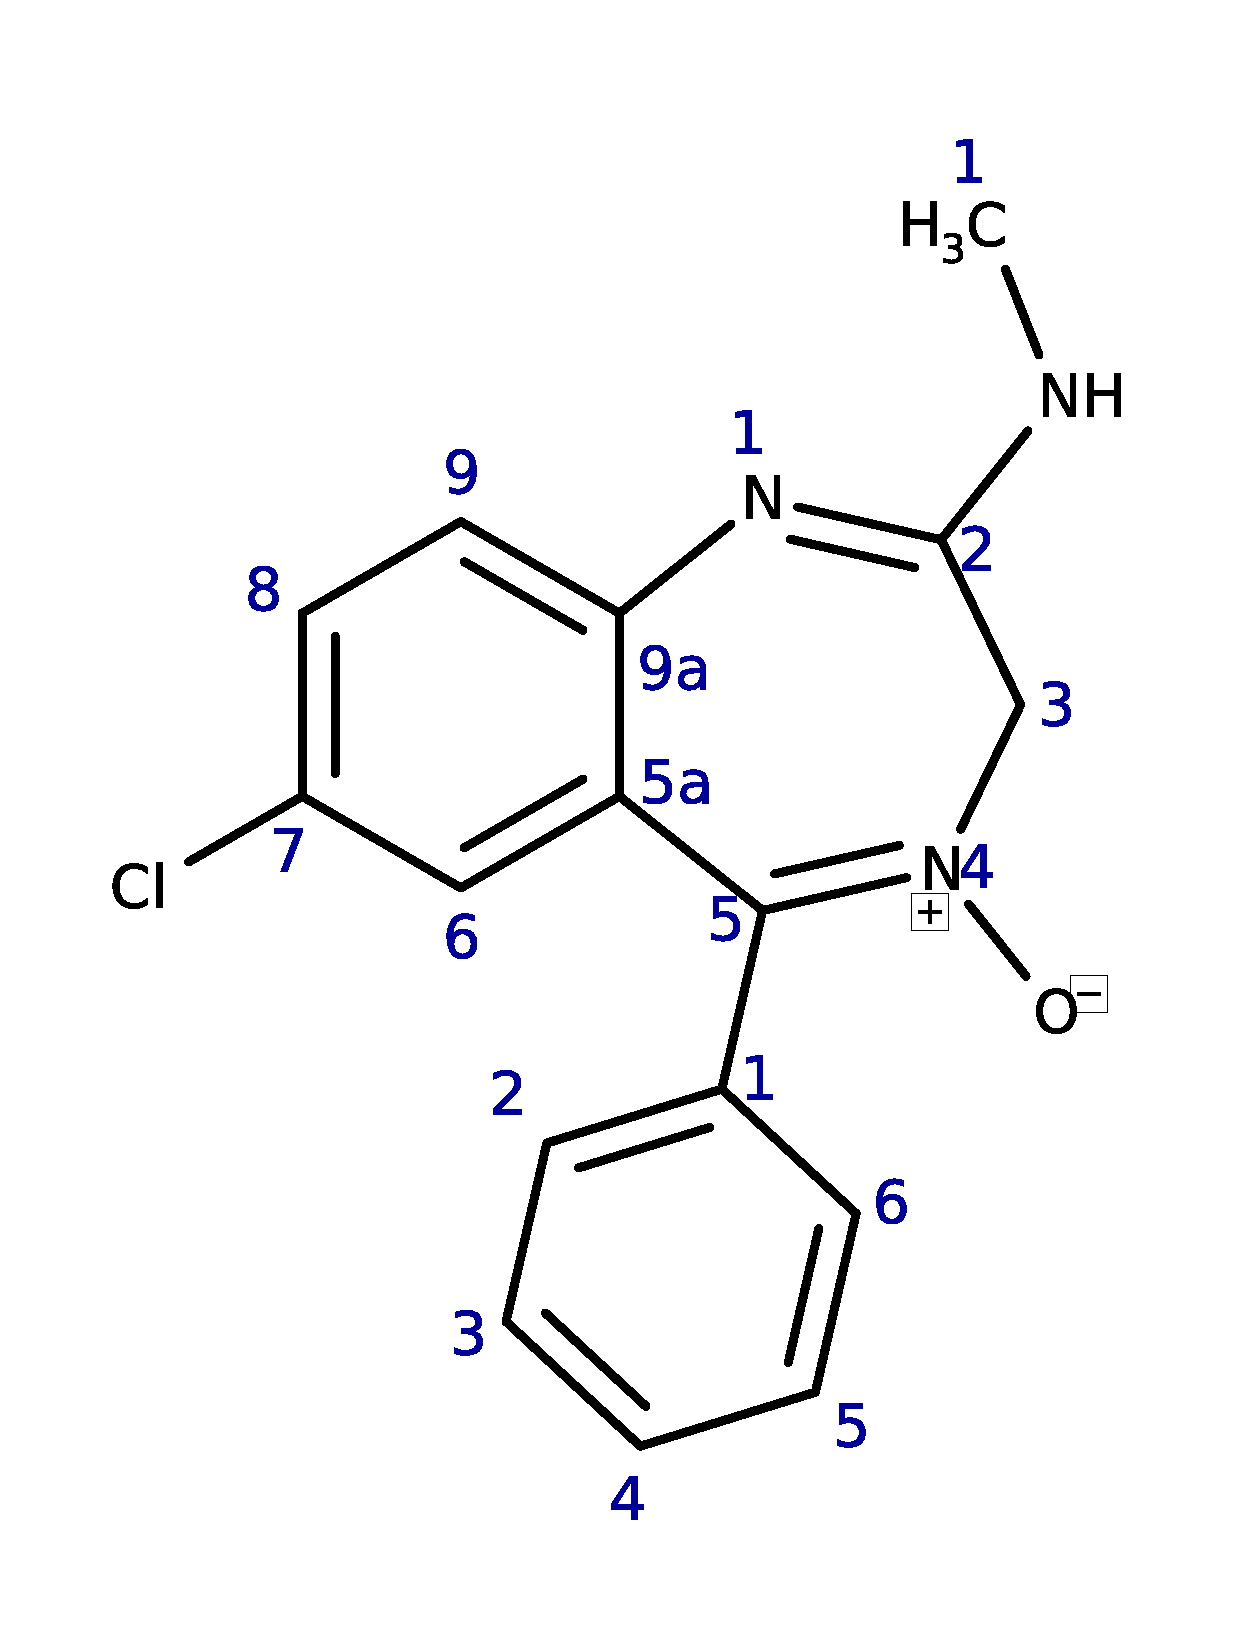
\includegraphics[width=\linewidth]{Chlordiazepoxide.pdf}
			\captionof{figure}{The structure of Chlordiazepoxide}
			\label{fig:cldiazepoxide}
		\end{minipage}
	\end{figure}

	\begin{figure}
		\centering
		\begin{minipage}{.5\textwidth}
			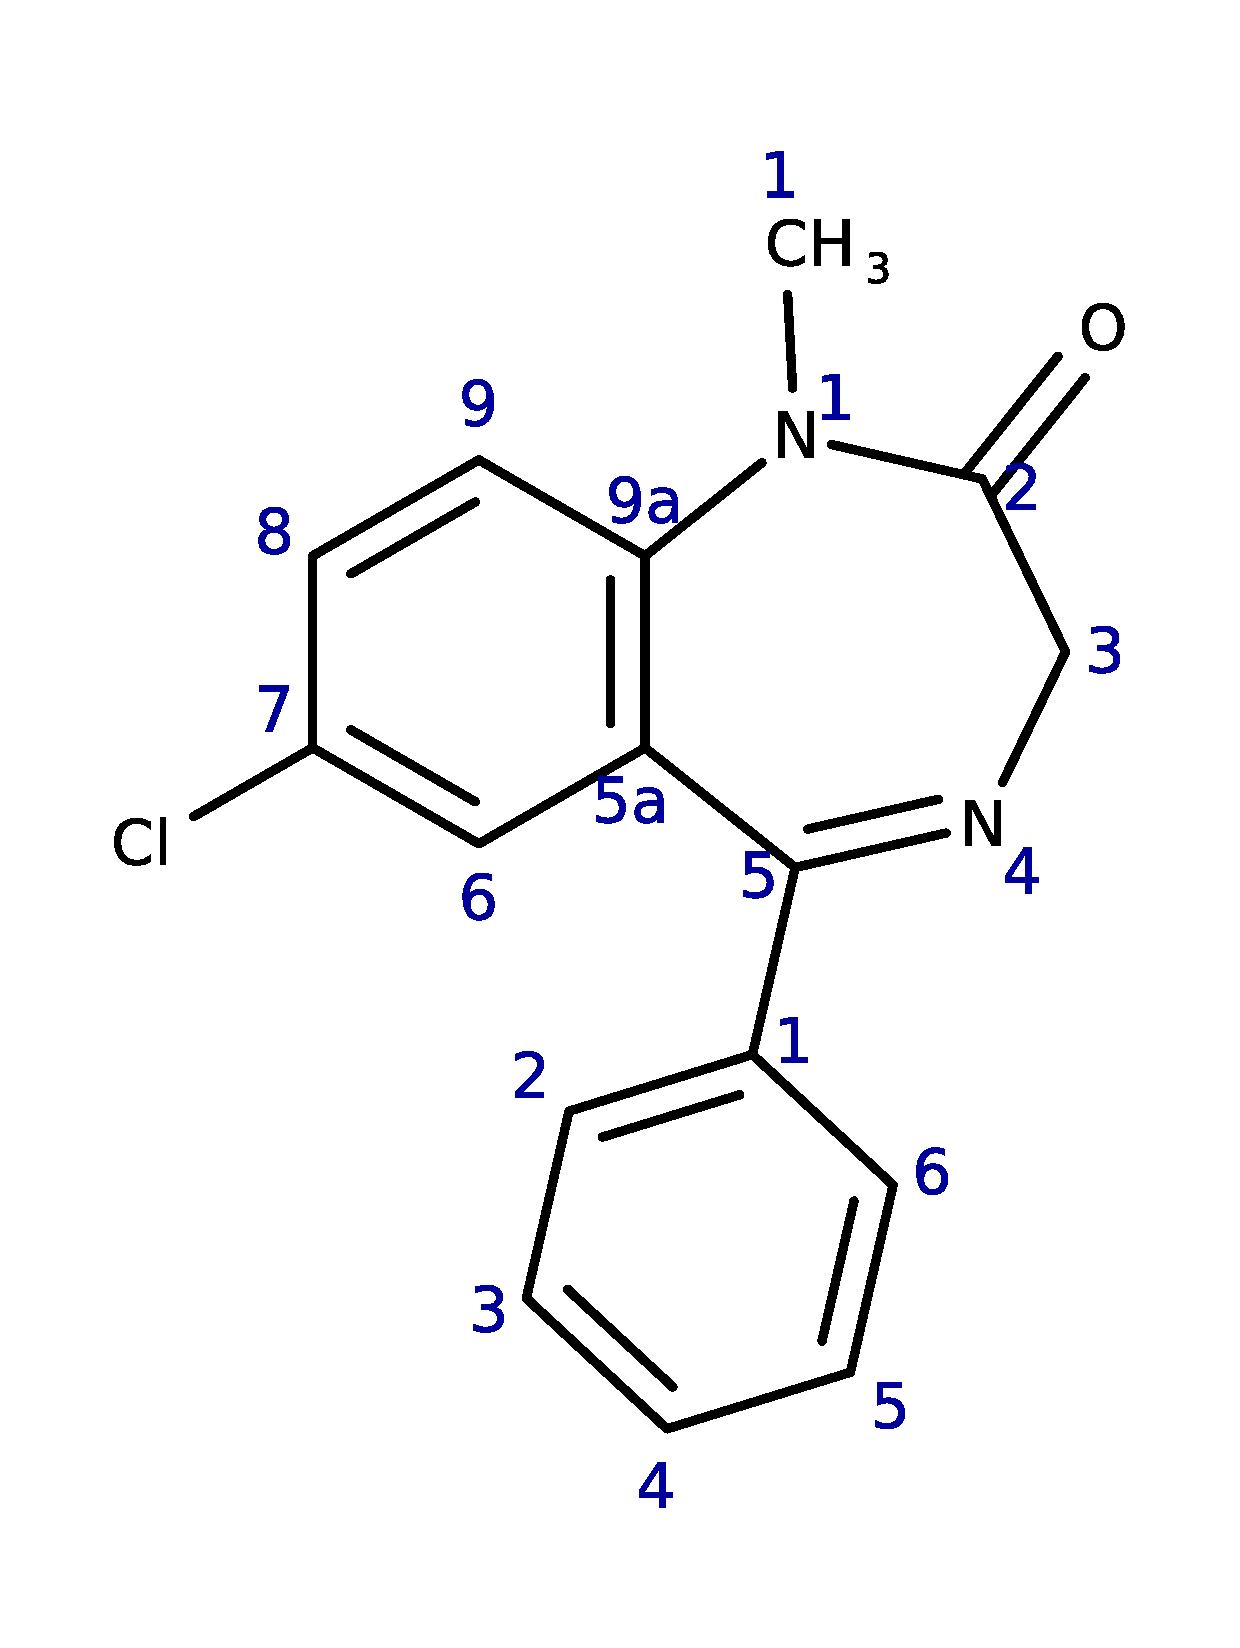
\includegraphics[width=\linewidth]{diazepam.pdf}
			\captionof{figure}{The structure of Diazepam}
			\label{fig:diazepam}
		\end{minipage}%
		\begin{minipage}{.5\textwidth}
			\centering
			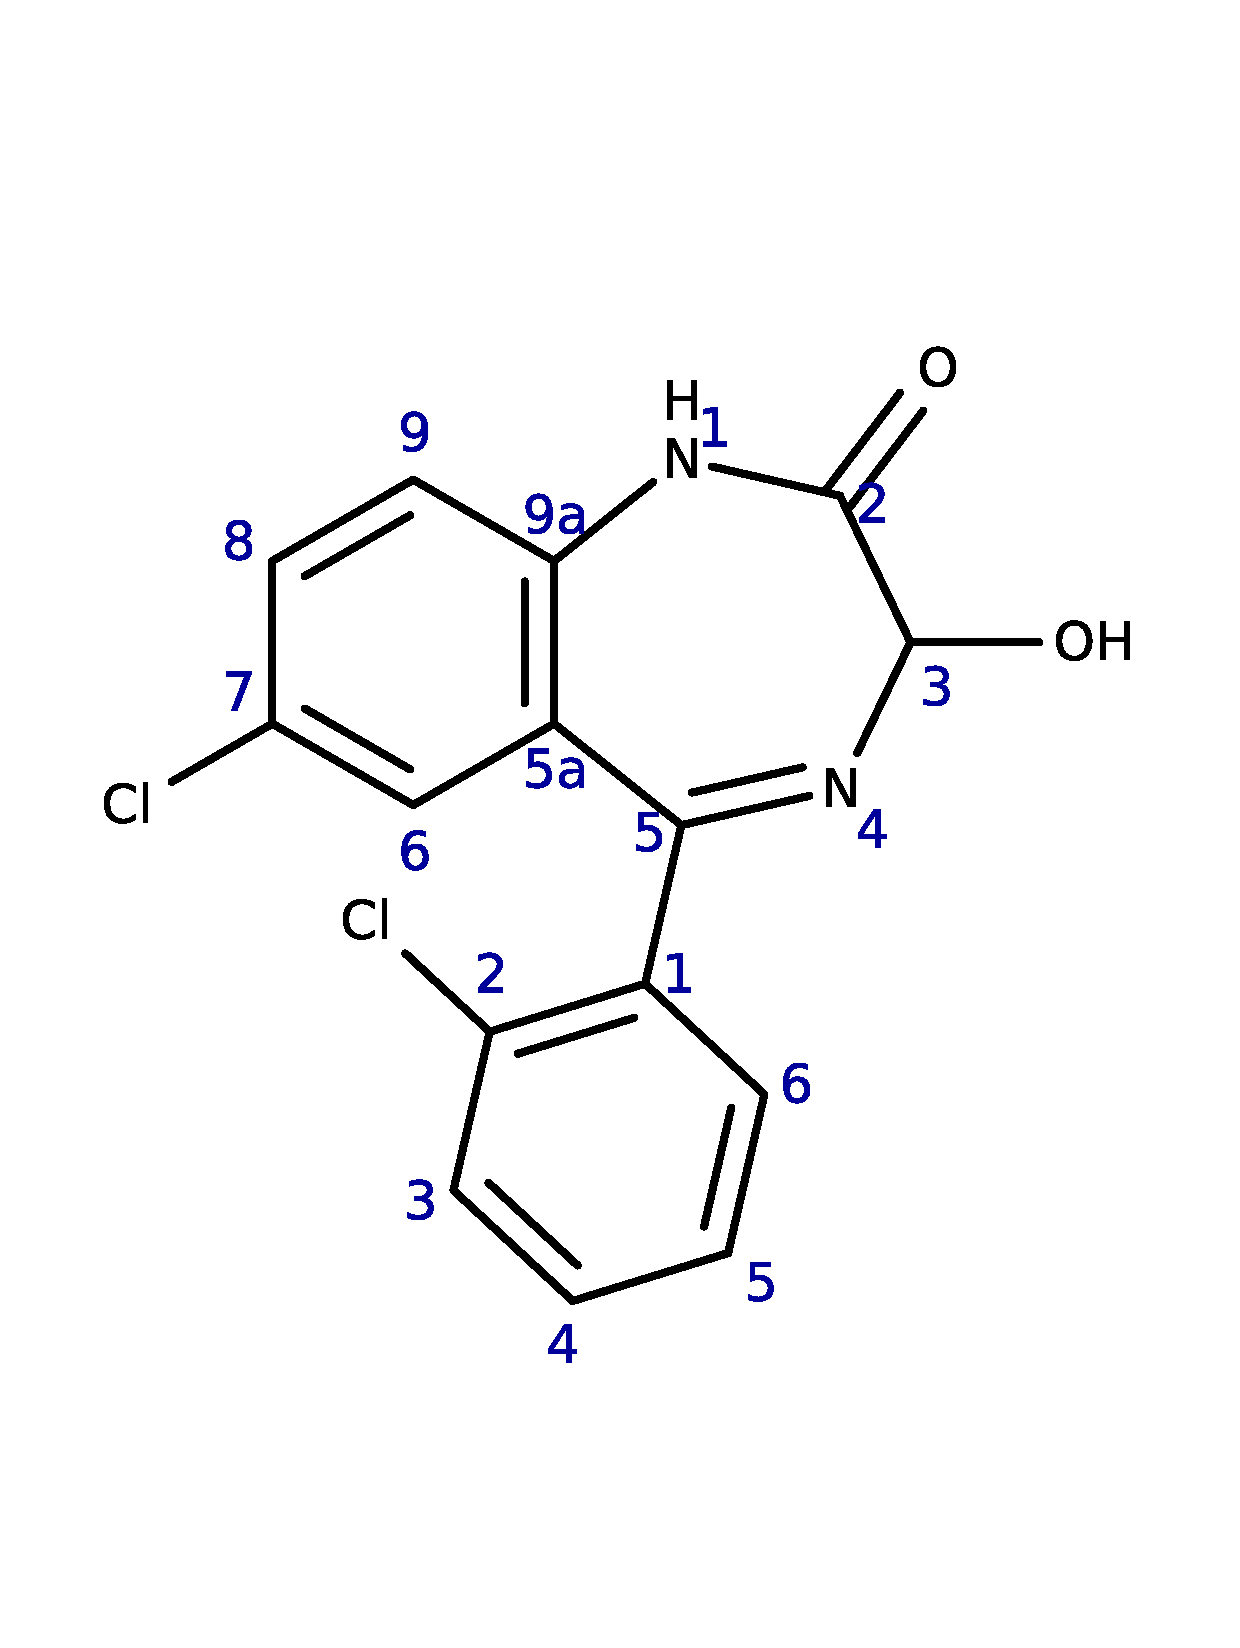
\includegraphics[width=\linewidth]{lorazapam.pdf}
			\captionof{figure}{The structure of Lorazepam}
			\label{fig:lorazepam}
		\end{minipage}

	\end{figure}
